\subsection{Classifying Graphs and Tournaments}
\label{sec:graphsandtournaments}

Let us look at how we can classify graphs and tournaments using \verb'orbiter'.
The program that we use is called \verb'graph.out' and it resides in 
\begin{quote}
\verb'ORBITER/SRC/APPS/GRAPH'\\
\end{quote}
The testing will take place in 
\begin{quote}
\verb'ORBITER/DATA/GRAPH_AND_TOURNAMENT'\\
\end{quote}
In this directory, the makefile allows us to classify graphs and tournaments 
on $n$ vertices, for small values of $n$. 
For instance, typing 
\begin{quote}
\verb'make g4'\\
\end{quote}
will produce the classification of graphs on $4$ vertices. 
The actual command is 
\begin{quote}
\verb'ORBITER/SRC/APPS/GRAPH/graph.out -n 4 -v 1'\\
\end{quote}
The output produced by this command contains the following lines:
\begin{quote}
Found 1 orbits at depth 6\\
0 : 1 orbits\\
1 : 1 orbits\\
2 : 2 orbits\\
3 : 3 orbits\\
4 : 2 orbits\\
5 : 1 orbits\\
6 : 1 orbits\\
total: 11\\
\end{quote}
This means that there are 11 graphs on 4 vertices in total, 
and that the number of graphs on $4$ vertices with $k$ edges is 
$$
\begin{array}{|c|*{7}{c|}}
\hline
k & 0 & 1 & 2 & 3 & 4 & 5 & 6 \\
\hline
\# \; \mbox{graphs} & 1 & 1 & 2 & 3 & 2 & 1 & 1 \\
\hline
\end{array}
$$
Of course, we could have noticed that the number of graphs with $k$ edges is the same as the number of graphs with ${n \choose 2} - k$ edges, which would 
have saved us a little bit. 
Next, we could run successively the commands
\begin{quote}
make g4\\
make g5\\
make g6\\
make g7\\
make g8\\
make g9\\
\end{quote}
to find out that the number of graphs with $n$ vertices is 
$$
\begin{array}{|c|*{9}{c|}}
\hline
n & 1 & 2 & 3 & 4 & 5 & 6 & 7 & 8 & 9  \\
\hline
\# \; \mbox{graphs} & 1 & 2 & 4 & 11 & 34 & 156 & 1044 & 12346 & 274668 \\
\hline
\end{array}
$$
which is nothing else than Sloan's sequence A000088 
(we have taken the freedom to fill in the values for $n=1,2,3$ by hand; these numbers are not difficult to come by). 
While it is well-known that we can use techniques from enumerative combinatorics 
to obtain these numbers, the point that is interesting to note is this: 
By issueing the commands above, we 
have actually {\em constructed} each of the graphs in the list.
If we were inclined to do so, we could look at these graphs and 
investigate them further. Of course, this would require us to 
gain a better understanding of how \verb'orbiter' maintains lists of orbits.

\bigskip

Let us have a closer look at the classification program. The relevant 
files are
\begin{quote}
\verb'ORBITER/SRC/APPS/GRAPH/graph.C'\\
\verb'ORBITER/SRC/APPS/GRAPH/graph.h'\\
\verb'ORBITER/SRC/APPS/GRAPH/graph_generator.C'\\
\end{quote}
Of these, \verb'graph.C' is the main program, \verb'graph.h' contains declarations, 
and \verb'graph_generator.C' defines a class with the same name (we generally 
rely of the convention that a class is defined in a file with the same name).
Let us have a look at the class \verb'graph_generator', which contains the following 
declarations (amongst others):
\begin{quote}
\verb'class graph_generator {'\\
\verb'public:'\\
  \verb'action *A_base; // symmetric group on n vertices'\\
  \verb'action *A_on_edges; // action on pairs'\\
\verb'};'\\
\end{quote}
These are pointers to objects of type action. 
An action is the way that permutation groups are defined in \verb'orbiter'.
The two actions \verb'A_base' and \verb'A_on_edges' correspond to the action on points 
and on edges, respectively. The first action is called \verb'A_base' because we consider this the basic action from which the other action is derived.
Looking into \verb'graph_generator.C', we see the following commands (inside the function \verb'graph_generator::init'):
\begin{quote}
\verb'A_base = new action;'\\
\verb'A_base->init_symmetric_group(n, verbose_level - 3);'\\
\end{quote}
The new command allocates memory for the action object. The command 
\verb'init_symmetric_group' makes \verb'A_base' become a symmetric group $\Sym_n$.  
In \verb'orbiter', this means that the group is acting on the numbers 
$0,1,\ldots,n-1.$
Regarding the second action, we find the commands
\begin{quote}
\verb'A_on_edges = new action;'\\
\verb'A_on_edges->induced_action_on_pairs(*A_base, A_base->Sims,'\\
\verb'  verbose_level - 3);'\\
\end{quote}
The first command allocates memory for the object.
The second command initialize the induced action of $\Sym_n$ 
on the set of unordered pairs. This means that \verb'A_on_edges' acts on 
the numbers $0,1,\ldots,{n\choose 2}-1.$
The identification with unordered pairs is according to the lexicographic ordering of 
subsets of size $2$:
$$
01, \; 02, \;03, \; \ldots, n-1,n. 
$$
% Thus
%\begin{eqnarray*}
%&0 = \{0,1\}, \; 1 = \{ 0,2\}, \; n-1=\{0,n-1\}, \\
%&n = \{1,2\}, \; 2 = \{1,3\},\ldots \\
%&{n \choose 2}-1 = \{n-2,n-1\}.
%\end{eqnarray*}
There are two reasons for working with two actions. 
First, it is more efficient to work with the group 
$\Sym_n$ acting on the vertices. This is what the action 
\verb'A_base' is for. 
The action \verb'A_on_edges' is the action of this group 
on unordered pairs, and graphs can be identified with orbits 
on subsets of pairs in this action. 
Thus, by classifying the orbits on subsets in this action, 
\verb'orbiter' will classify graphs on $n$ vertices. 
The size of the subset corresponds to the number of edges $k$ 
in the graph. 
The second reason for having the action \verb'A_base' 
around is the small degree of this action. 
As it turns out, permutation group algorithms are more efficient 
if small degree actions are used to represent the group.
For this reason, all arithmetic in $\Sym_n$ is done in the 
action on $n$ points. \verb'orbiter' uses the action \verb'A_on_edges' whenever it is classifying subsets,  
but maintains the group and group elements in the action \verb'A_base'. 

\bigskip

In case that we are classifying tournaments (directions of the 
complete graph $K_n$), we work with the action on ordered pairs, 
created using 
\begin{quote}
\verb'A_on_edges->induced_action_on_ordered_pairs(*A_base, '\\
\verb'  A_base->Sims, verbose_level - 3);'\\
\end{quote}
In this case, the pairs are ordered in such a way that 
each ordered pair appears together with the pair obtained 
by reversing the order. These pairs appear consecutively, 
and with the 
pair that lists the smaller element first preceeding the other pair. 
The lexicographic ordering of subsets is used to arrange the pairs.
So, the ordering of the $n(n-1)$ ordered pairs is
$$
01, \; 10, \; 02, \; 20, \; \;03, \; 30, \ldots, n-1,n, \;\; n,n-1. 
$$

\bigskip


Let us look at a specific example. Say we want to classify the 
graphs on $4$ vertices with $3$ edges. 
We run the command
\begin{quote}
\verb'ORBITER/SRC/APPS/GRAPH/graph.out -n 4 -v 1 -W'\\
\end{quote}
The option \verb'-W' means that the data that is computed is 
written to file. After completion, we find many files in 
the current directory. Let's look into the file 
\verb'graph_4_lvl_3' which contains representatives for the 
orbits on graphs with $4$ vertices and $3$ edges (slightly edited to better fit the page):
\begin{quote}
\verb'# 3'\\
\verb'3 0 1 2 6 aaaaaaadaaaaaaadaaaaaaaaaaaaaaabaaaaaaacaaaaaaab'\\
\verb'    aaaaaaadaaaaaaacaaabadacaaacabadaaadacab'\\
\verb'3 0 1 3 6 aaaaaaadaaaaaaacaaaaaaaaaaaaaaabaaaaaaacaaaaaaad'\\
\verb'    aaaaaaacaaaaaaabaaacabadabacaaad'\\
\verb'3 0 1 4 2 aaaaaaadaaaaaaabaaaaaaaaaaaaaaabaaaaaaacaaaaaaac'\\
\verb'    aaaaaaabaaaaaaababaaadac'\\
\verb'-1 3 4 in 0:00(6^2, 2) average is 4 + 2 / 3'\\
\end{quote}
What is this telling us? First of all, the file is somewhat hard to read for humans. 
It is a compromise between efficiency and machine readability. It is also 
a relict of a file format from an earlier program system, so there is a lagacy issue here.
The first row indicates that we have representatives of size $3$. 
The representatives are listed in the following three rows. 
Again, for some reason, each row starts by listing the size of the subset. 
Then, the subset is listed, followed by the order of the stabilizer. 
The remaining characters are an encoding of the generators for the stabilizer themselves, 
and are intended for machine processing. 
The row that starts with \verb'-1' lists (among other things that are not relevant at the moment) 
the number of representatives, and the distribution of group orders in parentheses. It also lists the average of all group orders.
So, the graphs on 4 vertices with $3$ edges are represented by 
$$
\begin{array}{|c|c|c|c|c|}
\hline
\mbox{Representative} & \mbox{Edges} & \mbox{Stabilizer Order} & \mbox{Description} & \mbox{Drawing}\\
\hline
\{0,1,2\} & \{01,02,03\} & 6 & 3\mbox{-Claw} & 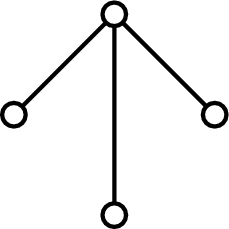
\includegraphics[width=15mm]{GRAPHICS/graph_4_3_0}\\
\{0,1,3\} & \{01,02,04\} & 6 & \mbox{Triangle} & 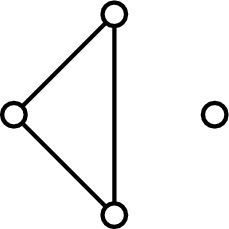
\includegraphics[width=15mm]{GRAPHICS/graph_4_3_1} \\
\{0,1,4\} & \{01,02,12\} & 2 & \mbox{Path}  & 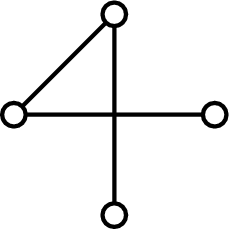
\includegraphics[width=15mm]{GRAPHICS/graph_4_3_2}\\
\hline
\end{array}
$$
In the drawings, the vertex numbered $0$ sits at the very top, and the ordering of vertices in counterclockwise.
We will follow this convention throughout the manual.
The average stabilizer order is $\frac{6+6+2}{3} = 4+\frac{2}{3}.$

\bigskip

Let us move on to the class of regular graphs. 
The command
\begin{quote}
\verb'make g8r3'\\
\end{quote}
which is an abbreviation for 
\begin{quote}
\verb'ORBITER/SRC/APPS/GRAPH/graph.out -n 8 -depth 12 -regular 3 -v 2 -W'\\
\end{quote}
classifies cubic graphs on $8$ vertices. We find $6$ graphs.
Reading the file
\begin{quote}
\verb'graph_8_r3_lvl_12'\\
\end{quote}
we find that these six graphs are represented by 
$$
\begin{array}{|c|c|c|}
\hline
\mbox{Representative} & \mbox{Stabilizer Order} &  \mbox{Drawing}\\
\hline
\{0, 1, 2, 7, 8, 13, 22, 23, 24, 25, 26, 27\}  & 1152 & 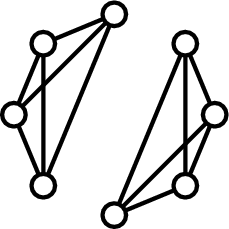
\includegraphics[width=15mm]{GRAPHICS/graph_8_r3_0}\\
\{0, 1, 2, 7, 8, 14, 19, 23, 24, 25, 26, 27\}  & 16 & 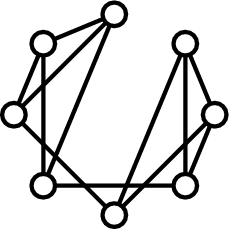
\includegraphics[width=15mm]{GRAPHICS/graph_8_r3_1}\\
\{0, 1, 2, 7, 9, 15, 18, 20, 24, 25, 26, 27\}  & 4 & 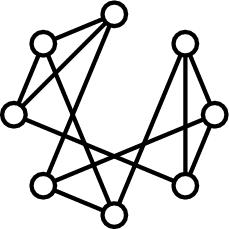
\includegraphics[width=15mm]{GRAPHICS/graph_8_r3_2}\\
\{0, 1, 2, 7, 9, 15, 20, 21, 23, 24, 25, 26\}  & 12 & 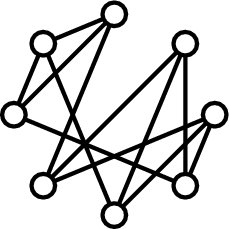
\includegraphics[width=15mm]{GRAPHICS/graph_8_r3_3}\\
\{0, 1, 2, 9, 10, 14, 16, 19, 20, 24, 26, 27\}  & 48 & 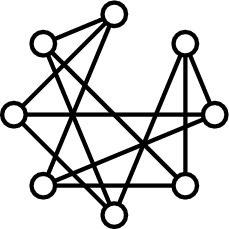
\includegraphics[width=15mm]{GRAPHICS/graph_8_r3_4}\\
\{0, 1, 2, 9, 10, 14, 16, 19, 21, 24, 25, 27\}  & 16 & 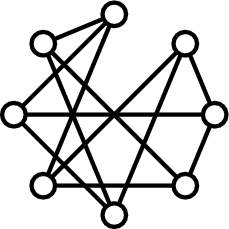
\includegraphics[width=15mm]{GRAPHICS/graph_8_r3_5}\\
\hline
\end{array}
$$
Of course, the drawings are not particularly nice. Thinking about the issue of how to draw a graph ``nicely'' leads us to contemplate what representatives are 
chosen for the graphs that we compute. The answer is that 
\verb'orbiter' always chooses the lexicographically least set in each orbit as representative. 
In addition, the representatives are listed in lexicographically increasing order. 


\bigskip

Next, let us have a look at tournaments. A tournament is a directed graph such that any two vertices 
are connected by exactly one directed edge (thus, a tournament is a direction of a complete graph). 
Let us classify tournaments with \verb'orbiter'.
The command 
\begin{quote}
\verb'make t4'\\
\end{quote}
which is an abbreviation for 
\begin{quote}
\verb'ORBITER/SRC/APPS/GRAPH/graph.out -n 4 -v 2 -tournament -W'\\
\end{quote}
classifies tournaments on $4$ vertices. 
The file \verb'tournament_4_lvl_6' contains the $4$ tournaments. They are:
$$
\begin{array}{|c|c|c|}
\hline
\mbox{Representative} & \mbox{Stabilizer Order} &  \mbox{Drawing}\\
\hline
\{0, 2, 4, 6, 8, 10\}  & 1 & 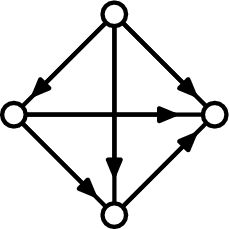
\includegraphics[width=25mm]{GRAPHICS/tournament_4_0}\\
\{0, 2, 4, 6, 9, 10\}  & 3 & 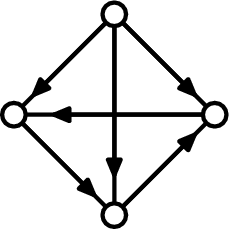
\includegraphics[width=25mm]{GRAPHICS/tournament_4_1}\\
\{0, 2, 5, 6, 8, 10\}  & 1 & 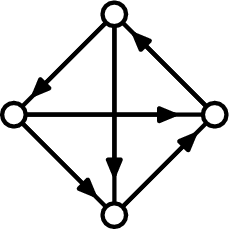
\includegraphics[width=25mm]{GRAPHICS/tournament_4_2}\\
\{0, 2, 5, 6, 8, 11\}  & 3 & 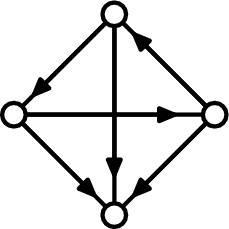
\includegraphics[width=25mm]{GRAPHICS/tournament_4_3}\\
\hline
\end{array}
$$

\bigskip

No piece in graph theory is complete without the unique graph on 10 vertices that is $3$-regular 
of girth $5$, better known as the Petersen graph. In \verb'orbiter', we issue the command
\begin{quote}
\verb'ORBITER/SRC/APPS/GRAPH/graph.out -n 10 -regular 3 -depth 15 '\\
\verb'    -girth 5 -v 2 -W'\\
\end{quote}
The file \verb'graph_10_r3_g5_lvl_15' is created (amongst many others), and contains the graph 
$$
\{0, 1, 2, 11, 12, 20, 21, 28, 29, 31, 33, 36, 38, 41, 42\}
$$
with an automorphism group of order $120$.
When drawn, this graph looks like this
$$
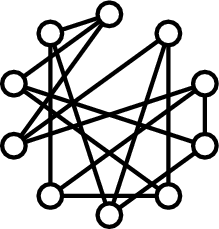
\includegraphics[width=35mm]{GRAPHICS/petersen}
$$
Of course, because of the lexicographic condition on the orbit representatives chosen, 
this is not the best drawing of this graph. 


\bigskip

This may be a good point to look at what \verb'orbiter' is really doing when we ask for the classification 
of a certain set of orbits. 
In a nutshell, the classification proceeds by establishing a tree. 
The nodes of the tree are the orbits on ``partial sets.'' 
The definition of partial sets depends on the problem at hand. 
In the example of classifying graphs, we can think of the partial objects as graphs with fewer edges satisfying 
the natural induced conditions. 
A descendant $B$ of a node $A$ is a subset $B$ that contains $A$. 
An immediate descendant is a descendant whose size is exactly one larger than the previous set. 
Thus, $B$ is an immediate descendant of $A$ if $A \subseteq B$ and $|B \setminus A| = 1$.
We can draw the tree in such a way that the root node (corresponding to the empty set) 
is at the very top, and so that the descendants are below the node from which they originate, connected to 
that node by an edge. 
In the case of the Petersen graph, this tree has $460$ nodes and looks like this:
$$
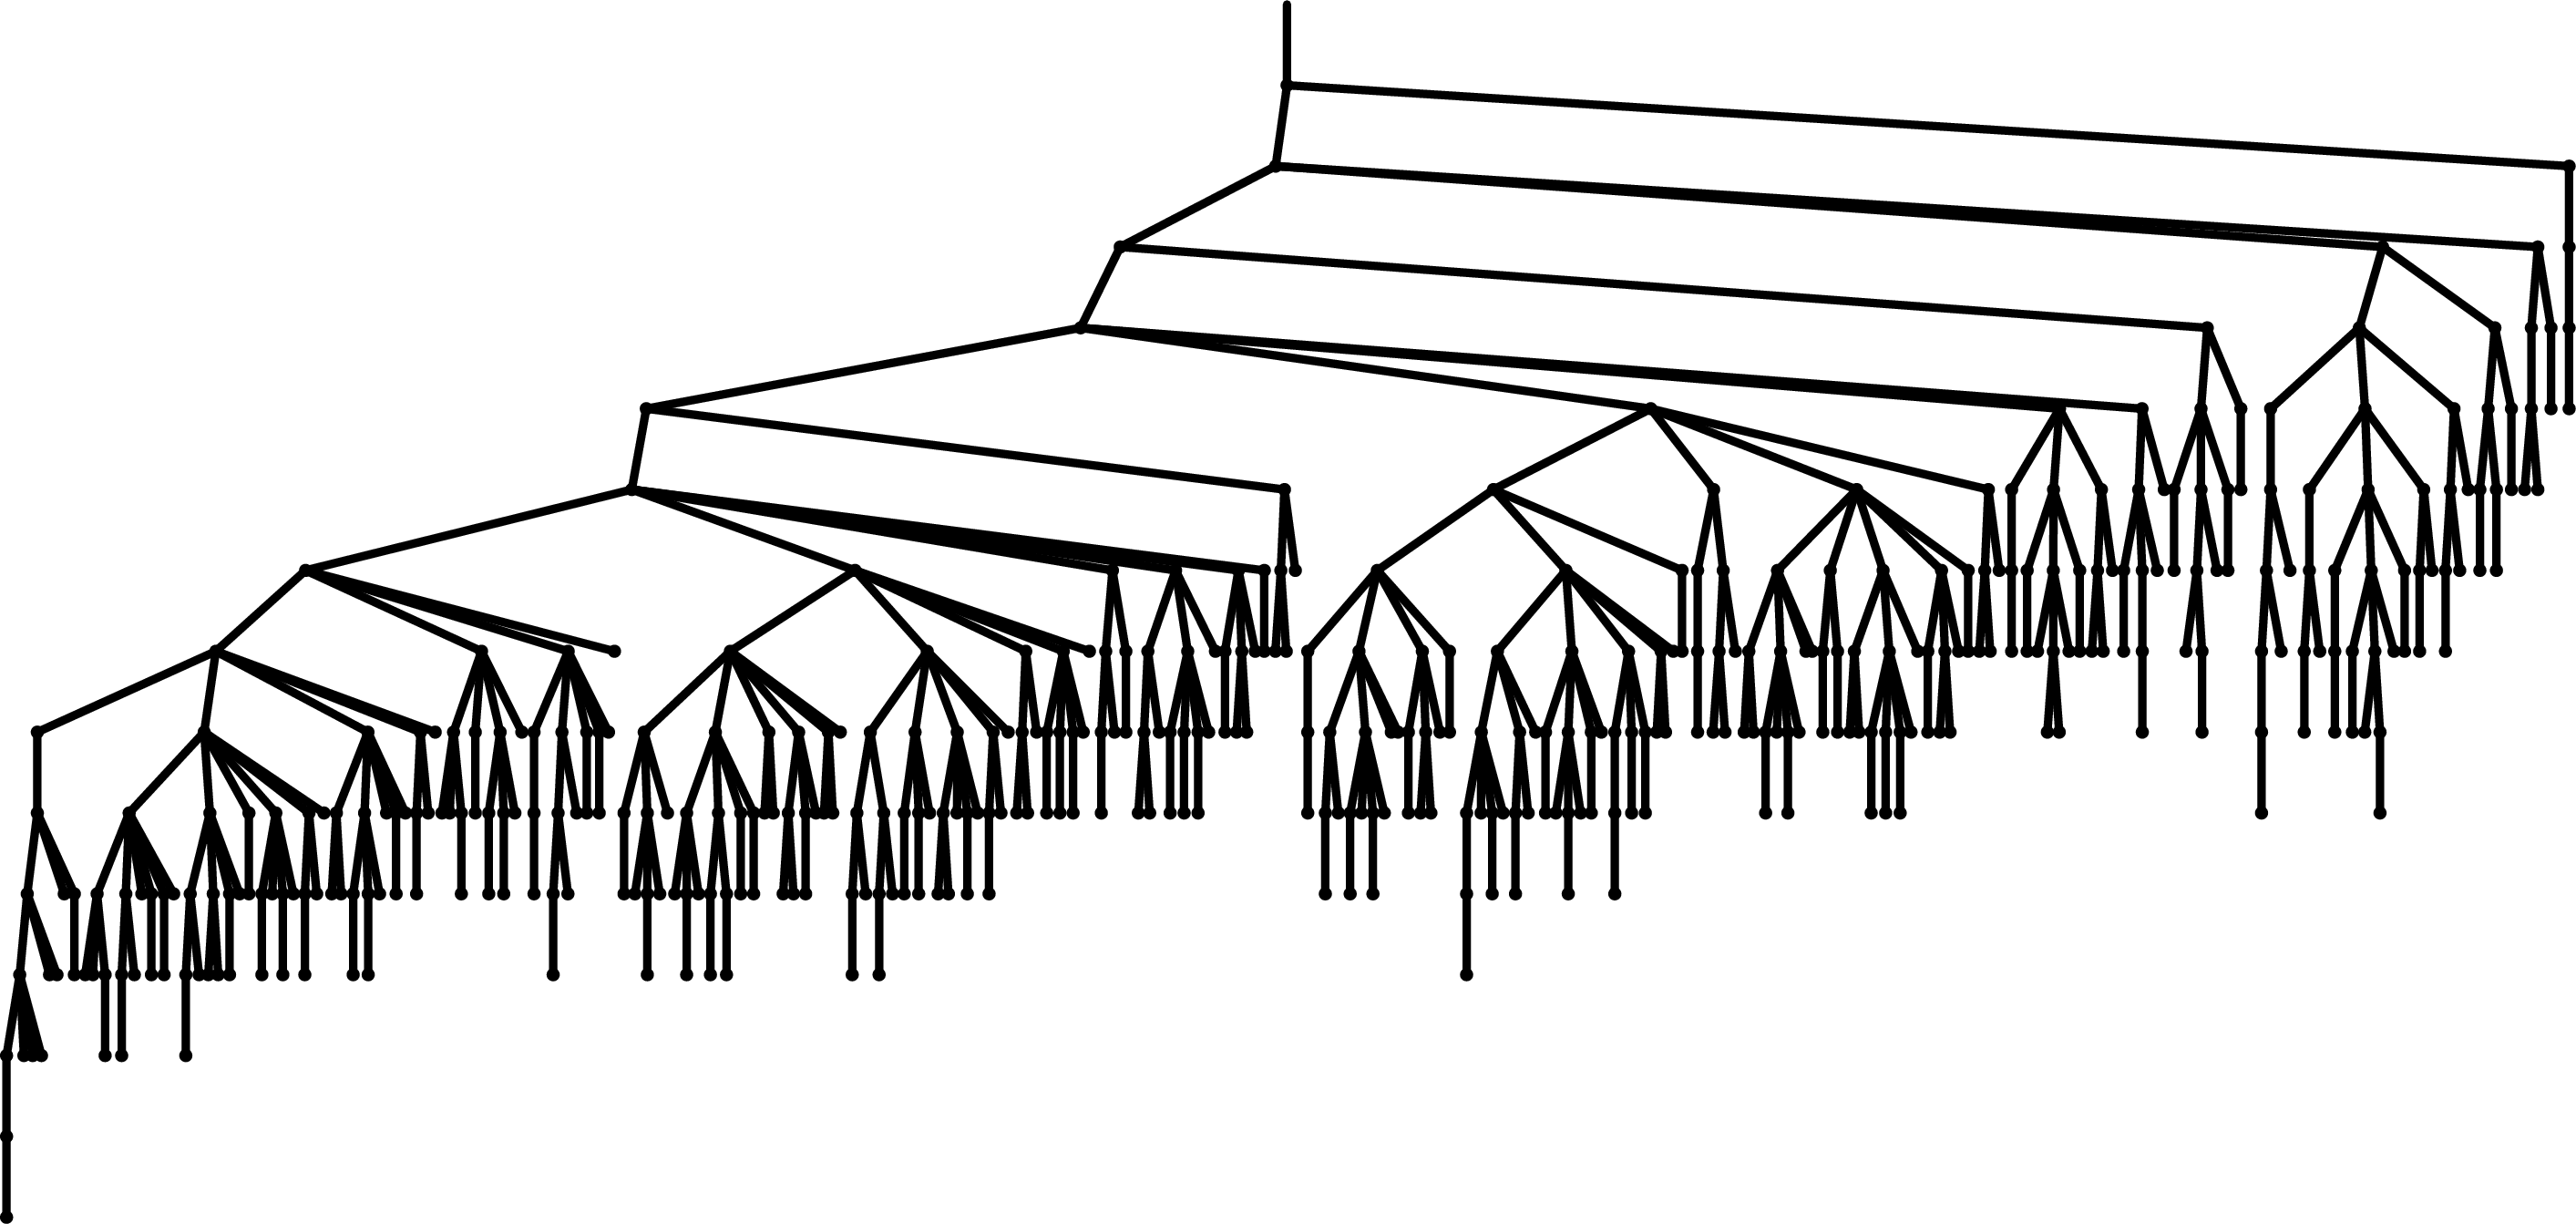
\includegraphics[width=150mm]{GRAPHICS/petersen_tree}
$$
The Petersen graph itself is represented by the node that is at the very bottom and at the very left.
The graphs represented in this tree have the property that they are defined on 10 vertices, 
each vertex has degree at most 3, and they contain no cycles of length less than $5$.
For each orbit of this kind of graph, the lexicographically least representation is chosen.

\bigskip

Let us look at the structure of the class \verb'graph_generator'.
In it, we find the declaration 
\begin{quote}
\verb'generator *gen;'
\end{quote}
The \verb'orbiter' 
class \verb'generator' is responsible for classifying orbits of a group.
To initialize, we find in the function \verb'graph_generator::init' 
the call
\begin{quote}
\verb'gen->initialize(A_base, A_on_edges,  '\\
\verb'    A_base->strong_generators, A_base->tl, '\\
\verb'    target_depth, '\\
\verb'    prefix, verbose_level - 1);'\\
\end{quote}
As pointed out above, the first two arguments \verb'A_base' and 
\verb'A_on_edges' represent the permutation group whose orbits 
on subsets we plan to classify. 
The next two arguments \verb'A_base->strong_generators' 
and \verb'A_base->tl' represent the actual generating system 
for the group. The argument \verb'target_depth' is a variable that 
has been computed previously to represent the size of subsets that 
we wish to classify. It depends on the type of graph or tournament 
that we specified using the command line arguments.
The argument \verb'prefix' is the prefix for the name of the output files. 
The last argument \verb'verbose_level - 1' specifies how 
verbose the function \verb'initialize' be during its processing.

\bigskip

In order to get started, we also need to specify the conditions that 
we want to impose on the subsets. 
These conditions depend on the type of graph or tournament that we 
wish to classify, and the specifics have been determined by command line arguments. 
Instead of going into all the details, let us just distinguish the 
case of graphs and the case of tournaments. 
In both cases, we inform the class \verb'generator' of a test function. 
This is done by means of a function pointer.
So, we find the command 
\begin{quote}
\verb'gen->init_check_func(::check_conditions, '\\
\verb'    (void *)this /* candidate_check_data */);'\\
\end{quote}
which informs \verb'generator' of the presence of the function 
\verb'::check_conditions'. This test function is a global function 
because function pointers are a feature of C, and they can only be 
pointers to gloabl functions, not member functions of a class.
This leaves the issue of telling the global test function
the instance of the class \verb'graph_generator'. 
This is done by means of a void pointer. This is a pointer that 
is declared to be of type void, and that is passed to the class 
\verb'generator'. Whenever the instance of \verb'generator'
wishes to call the test function, it passes the data pointer as an extra argument. 
The test function then takes this argument and type casts it to 
the appropriate type (here \verb'my_generator'), and issues the 
call of the appropriate member function. 
Here is the definition of the global test function:
\begin{quote}
\verb'INT check_conditions(ostream &ost, INT len, INT *S, '\\
\verb'    void *data, INT verbose_level)'\\
\verb'{'\\
\verb'    graph_generator *Gen = (graph_generator *) data;'\\
\verb''\\
\verb'    if (Gen->f_tournament) {'\\
\verb'        return Gen->check_conditions_tournament(len, S, verbose_level);'\\
\verb'        }'\\
\verb'    else {'\\
\verb'        return Gen->check_conditions(len, S, verbose_level);'\\
\verb'    }'\\
\verb'}'\\
\end{quote}
As we can see, the void pointer \verb'data' is the fourth argument. 
The second and thir argument are the set that we wish to test. 
It is simply a vector \verb'S' of integers of length \verb'len'.
The first argument can be ignored. The last argument specifies the 
verboseness of the test function. 
The line 
\begin{quote}
\verb'graph_generator *Gen = (graph_generator *) data;'\\
\end{quote}
is the cast of the void pointer \verb'data' to a pointer to an object 
of type \verb'graph_generator'.
This is so that the test function can then call the appropriate member functions 
of the class \verb'graph_generator' to perform the actual testing.

